\documentclass[12pt, twoside]{book}
%\documentclass[12pt, oneside]{book}  % jednostranna tlac

%spravne nastavenie okrajov
\usepackage[a4paper,top=2.5cm,bottom=2.5cm,left=3.5cm,right=2cm]{geometry}
%zapnutie fontov pre UTF8 kodovanie
\usepackage[utf8]{inputenc}
\usepackage[T1]{fontenc}

%zapnutie slovenskeho delenia slov
%a automatickych nadpisov ako Obsah, Obrázok a pod. v slovencine
\usepackage[slovak]{babel} % vypnite pre prace v anglictine!

%nastavenie riadkovania podla smernice
\linespread{1.25} % hodnota 1.25 by mala zodpovedat 1.5 riadkovaniu

% balicek na vkladanie zdrojoveho kodu
\usepackage{listings}
% ukazky kodu su cislovane ako Listing 1,2,...
% tu je Listing zmenene na Algoritmus 1,2,...
\renewcommand{\lstlistingname}{Algoritmus}
% nastavenia balicka listings
% mozete pridat aj language=...
% na nastavenie najcastejsie pouzivaneho prog. jazyka
% takisto sa da zapnut cislovanie riadkov
\lstset{frame=lines}

% balicek na vkladanie obrazkov
\usepackage{graphicx}
% balicek na vkladanie celych pdf dokumentov, tu zadanie
\usepackage{pdfpages}
% balicek na spravne formatovanie URL
\usepackage{url}
% balicek na hyperlinky v ramci dokumentu
% zrusime farebne ramiky okolo liniek aby pdf
% vyzeralo rovnako ako tlacena verzia
\usepackage[hidelinks,breaklinks]{hyperref}



% -------------------
% --- Definicia zakladnych pojmov
% --- Vyplnte podla vasho zadania, rok ma byt rok odovzdania
% -------------------
\def\mfrok{2024}
\def\mfnazov{Sémantická podobnosť textov v slovenskom jazyku}
\def\mftyp{Bakalárska práca}
\def\mfautor{Matej Krajčovič}
\def\mfskolitel{Lukáš Radoský}

%ak mate konzultanta, odkomentujte aj jeho meno na titulnom liste
\def\mfkonzultant{tit. Meno Priezvisko, tit. }  

\def\mfmiesto{Bratislava, \mfrok}

% študenti BIN a DAV odkomentujú príslušnú dvojicu riadkov
\def\mfodbor{ Informatika}
\def\program{ Aplikovaná informatika}
% pre BIN:
%\def\mfodbor{ Informatika a Biológia }
%\def\program{ Bioinformatika }
% pre DAV:
%\def\mfodbor{ Informatika a Matematika } 
%\def\program{ Dátová veda }

% Ak je školiteľ z FMFI, uvádzate katedru školiteľa, zrejme by mala byť aj na zadaní z AIS2
% Ak máte externého školiteľa, uvádzajte Katedru informatiky 
\def\mfpracovisko{ Katedra Aplikovanej informatiky }

\begin{document}    
\frontmatter
\pagestyle{empty}

% -------------------
% --- Obalka ------
% -------------------

\begin{center}
\sc\large
Univerzita Komenského v Bratislave\\
Fakulta matematiky, fyziky a informatiky

\vfill

{\LARGE\mfnazov}\\
\mftyp
\end{center}

\vfill

{\sc\large 
\noindent \mfrok\\
\mfautor
}

\cleardoublepage
% --- koniec obalky ----

% -------------------
% --- Titulný list
% -------------------


\noindent

\begin{center}
\sc  
\large
Univerzita Komenského v Bratislave\\
Fakulta matematiky, fyziky a informatiky

\vfill

{\LARGE\mfnazov}\\
\mftyp
\end{center}

\vfill

\noindent
\begin{tabular}{ll}
Študijný program: & \program \\
Študijný odbor: & \mfodbor \\
Školiace pracovisko: & \mfpracovisko \\
Školiteľ: & \mfskolitel \\
% Konzultant: & \mfkonzultant \\
\end{tabular}

\vfill


\noindent \mfmiesto\\
\mfautor

\cleardoublepage
% --- Koniec titulnej strany


% -------------------
% --- Zadanie z AIS
% -------------------
% v tlačenej verzii s podpismi zainteresovaných osôb.
% v elektronickej verzii sa zverejňuje zadanie bez podpisov
% v pracach v angličtine anglické aj slovenské zadanie

\newpage 
\setcounter{page}{2}
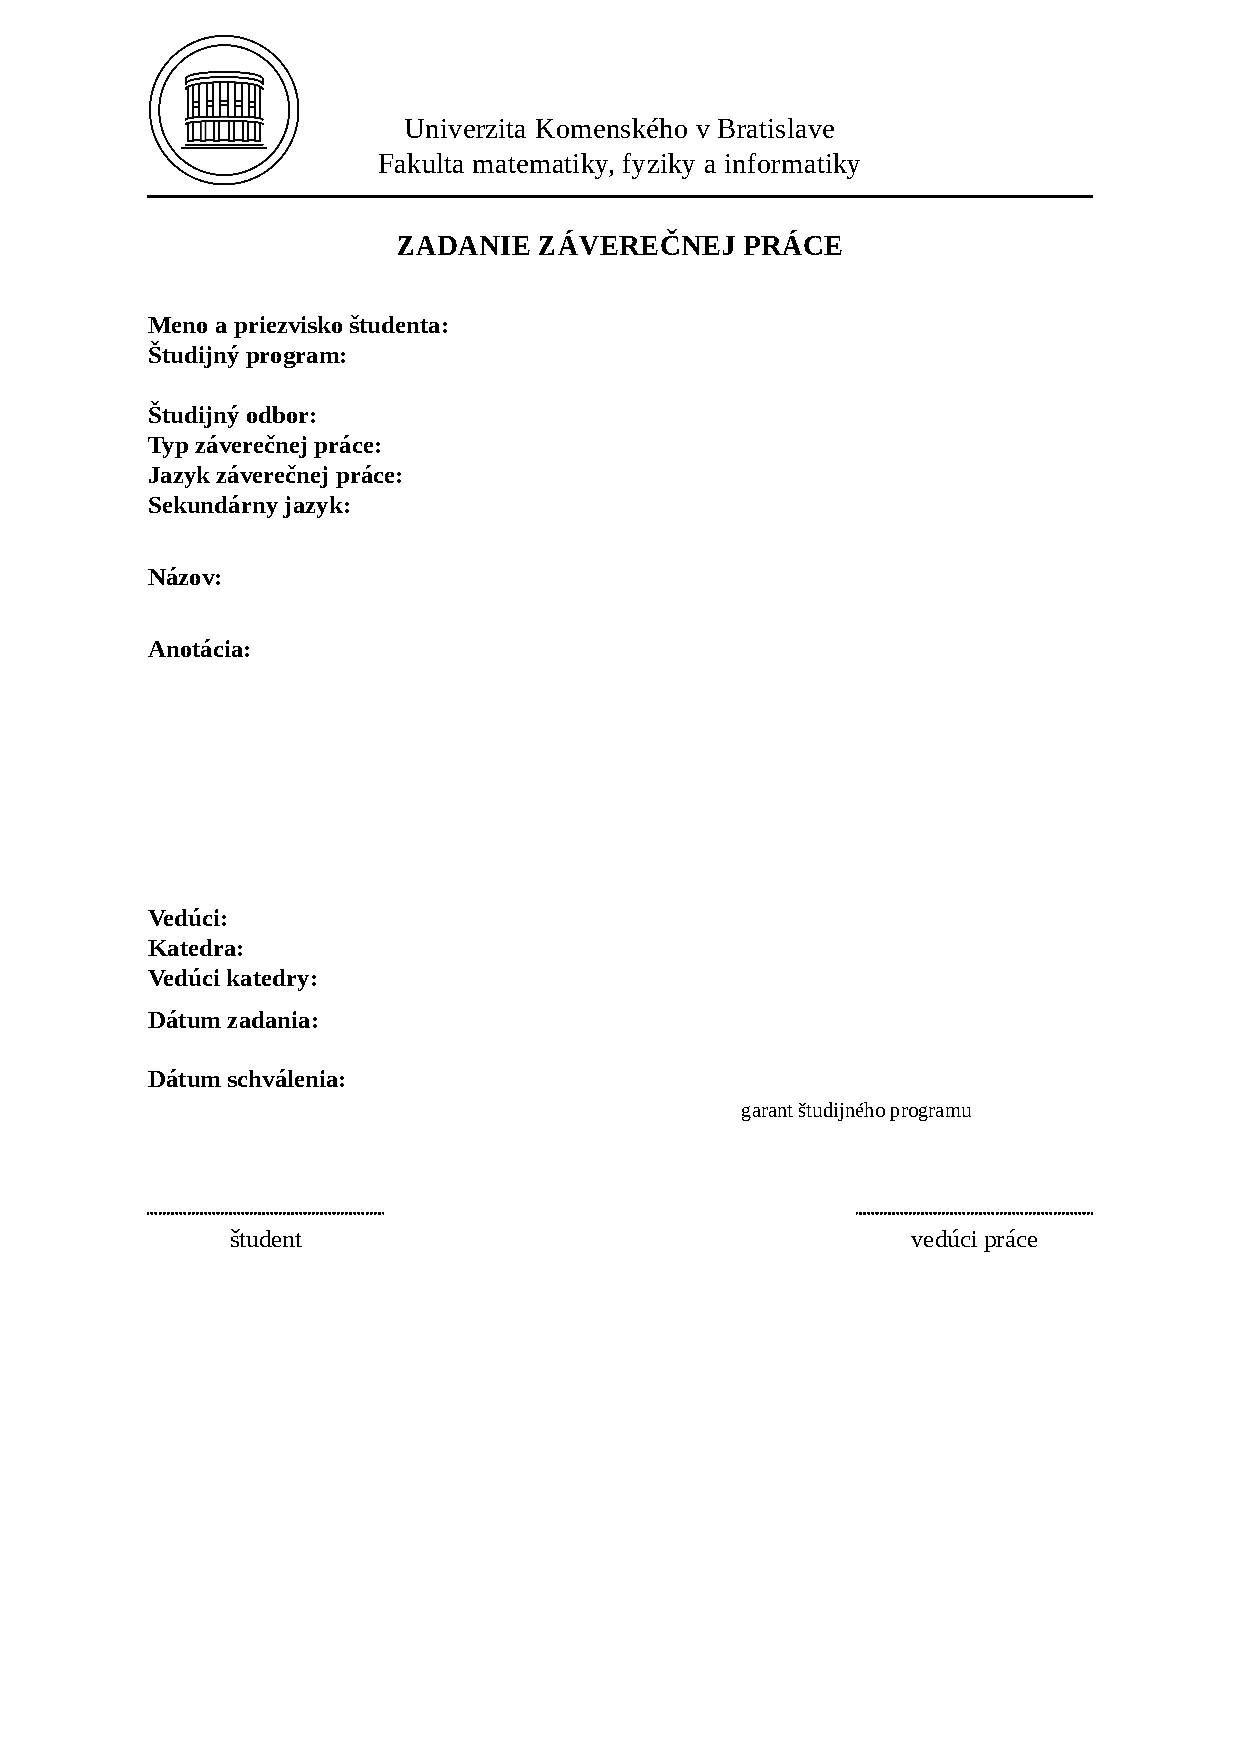
\includepdf{images/zadanie.pdf}

% --- Koniec zadania


% -------------------
%   Poďakovanie - nepovinné
% -------------------
\newpage 
\pagestyle{plain}
~

\vfill
{\bf Poďakovanie:} Chcel by som poďakovať svojmu školiteľovi, Lukášovi Radoskému, za jeho pomoc a podporu počas zhotovovania mojej práce. 

% --- Koniec poďakovania

% -------------------
%   Abstrakt - Slovensky
% -------------------
\newpage 
\section*{Abstrakt}

Táto práca sa zaoberá analýzou a porovnaním rôznych metód určovania sémantickej podobnosti textov v slovenskom jazyku. V práci sú predstavené a testované tri modely: Text-embedding-ada-002, SlovakBert a Paraphrase-multilingual-mpnet-base-v2, ktoré boli použité na tri vybrané dátové sady. Cieľom práce bolo zistiť, ktorý z modelov poskytuje najpresnejšie výsledky pri analýze sémantickej podobnosti slovenských textov. Výsledky ukázali, že model Text-embedding-ada-002 preukázal konzistentnú výkonnosť naprieč všetkými datasetmi, zatiaľ čo SlovakBert vyžaduje ďalšie špecifické trénovanie na zlepšenie jeho výkonu. Model Paraphrase-multilingual-mpnet-base-v2 zase vykázal výborné výsledky na datasete SemEval-2015-example\_sk, ale jeho úplné schopnosti neboli možné testovať kvôli obmedzeniam platených služieb. Práca poskytuje základ pre ďalší vývoj a zlepšenie modelov pre sémantickú analýzu textov v slovenskom jazyku.


\paragraph*{Kľúčové slová:} sémantická podobnosť textov, strojové učenie, rozsiahle jazykové modely, umelá inteligencia, slovenský jazyk
% --- Koniec Abstrakt - Slovensky


% -------------------
% --- Abstrakt - Anglicky 
% -------------------
\newpage 
\section*{Abstract}

This thesis deals with the analysis and comparison of different methods of determining the semantic similarity of texts in the Slovak language. Three models are present and test in this thesis: Text-embedding-ada-002, SlovakBert and Paraphrase-multilingual-mpnet-base-v2, which were used on three selected data sets. The aim was to evaluate which of the models provides the most accurate results when analyzing the semantic similarity of Slovak texts. The results showed that the Text-embedding-ada-002 model demonstrated consistent performance across all datasets, while SlovakBert requires additional specific training to improve its performance. The Paraphrase-multilingual-mpnet-base-v2 model, on the other hand, showed excellent results on the SemEval-2015-example\_sk dataset, but its full capabilities could not be tested due to the limitations of paid services. The work provides a basis for further development and improvement of models for the semantic analysis of texts in the Slovak language.


\paragraph*{Keywords:} semantic similarity of texts, machine learning, extensive language models, artificial intelligence, Slovak language

% --- Koniec Abstrakt - Anglicky

% -------------------
% --- Predhovor - v informatike sa zvacsa nepouziva
% -------------------
%\newpage 
%
%\chapter*{Predhovor}
%
%Predhovor je všeobecná informácia o práci, obsahuje hlavnú charakteristiku práce 
%a okolnosti jej vzniku. Autor zdôvodní výber témy, stručne informuje o cieľoch 
%a význame práce, spomenie domáci a zahraničný kontext, komu je práca určená, 
%použité metódy, stav poznania; autor stručne charakterizuje svoj prístup a svoje 
%hľadisko. 
%
% --- Koniec Predhovor


% -------------------
% --- Obsah
% -------------------

%\newpage 

\tableofcontents

% ---  Koniec Obsahu

% -------------------
% --- Zoznamy tabuliek, obrázkov - nepovinne
% -------------------

%\newpage 

%\listoffigures
\listoftables

% ---  Koniec Zoznamov

\mainmatter
\pagestyle{headings}


\input uvod.tex 

\input kapitola.tex

\input zaver.tex

% -------------------
% --- Bibliografia
% -------------------


%\newpage	

\backmatter

\thispagestyle{empty}
\clearpage

\bibliographystyle{plain}
\bibliography{literatura} 

%Prípadne môžete napísať literatúru priamo tu
%\begin{thebibliography}{5}
 
%\bibitem{br1} MOLINA H. G. - ULLMAN J. D. - WIDOM J., 2002, Database Systems, Upper Saddle River : Prentice-Hall, 2002, 1119 s., Pearson International edition, 0-13-098043-9

%\bibitem{br2} MOLINA H. G. - ULLMAN J. D. - WIDOM J., 2000 , Databasse System implementation, New Jersey : Prentice-Hall, 2000, 653s., ???

%\bibitem{br3} ULLMAN J. D. - WIDOM J., 1997, A First Course in Database Systems, New Jersey : Prentice-Hall, 1997, 470s., 

%\bibitem{br4} PREFUSE, 2007, The Prefuse visualization toolkit,  [online] Dostupné na internete: <http://prefuse.org/>

%\bibitem{br5} PREFUSE Forum, Sourceforge - Prefuse Forum,  [online] Dostupné na internete: <http://sourceforge.net/projects/prefuse/>

%\end{thebibliography}

%---koniec Referencii

% -------------------
%--- Prilohy---
% -------------------

%Nepovinná časť prílohy obsahuje materiály, ktoré neboli zaradené priamo  do textu. Každá príloha sa začína na novej strane.
%Zoznam príloh je súčasťou obsahu.
%

\end{document}






